\documentclass[aspectratio=169, 11pt]{beamer}

% Packages
\usepackage[utf8]{inputenc}
\usepackage{amsmath, amssymb, amsfonts}
\usepackage{graphicx}
\usepackage{booktabs}
\usepackage{ragged2e}
\usepackage{minted}
\usepackage{xcolor}
\usepackage{tikz}
\usepackage{algorithm}
\usepackage{algorithmic}
\usepackage{listings}
\usepackage{tcolorbox}

\usetikzlibrary{arrows.meta,positioning,fit,shapes.symbols}
\usetikzlibrary{arrows,shapes}
\definecolor{LightGray}{gray}{0.975}
\definecolor{links}{HTML}{2A1B81}
\hypersetup{colorlinks,linkcolor=,urlcolor=blue}
\AtBeginEnvironment{minted}{%
    \renewcommand{\fcolorbox}[4][]{#4}
}

\title[Classification]{ML101 \\ Lecture 04: Classification}
\subtitle{An Introduction to Statistical Learning}
\author{James, Witten, Hastie \& Tibshirani}
\date{\today}

% Remove navigation symbols...
\setbeamertemplate{navigation symbols}{}

\defbeamertemplate*{footline}{shadow theme}{
    \leavevmode
    \hbox{
        \begin{beamercolorbox}[
                wd =        0.33\paperwidth,
                ht =        2.5ex,
                dp =        1.125ex,
                leftskip =  0.3cm plus1fil,
                rightskip = 0.3cm
            ]{author in head/foot}
            \flushleft ML101
        \end{beamercolorbox}
        \begin{beamercolorbox}[
                wd =        0.33\paperwidth,
                ht =        2.5ex,
                dp =        1.125ex,
                leftskip =  0.3cm plus1fil,
                rightskip = 0.3cm
            ]{author in head/foot}
            \insertshorttitle
        \end{beamercolorbox}
        \begin{beamercolorbox}[
                wd =        0.33\paperwidth,
                ht =        2.5ex,
                dp =        1.125ex,
                leftskip =  0.3cm plus1fil,
                rightskip = 0.3cm
            ]{title in head/foot}
            \hfill \insertframenumber\,/\,\inserttotalframenumber%
        \end{beamercolorbox}
    }
}

\AtBeginSection[]
{
     \begin{frame}<beamer>
     \frametitle{Plan}
     \tableofcontents[currentsection]
     \end{frame}
}

\usefonttheme{serif}

\newcommand\Wider[2][18mm]{%
    \makebox[\linewidth][c]{%
        \begin{minipage}{\dimexpr\textwidth+#1\relax}
            \raggedright#2
        \end{minipage}%
    }%
}
\newcommand\userinput[1]{\textbf{#1}}

\begin{document}

\frame{\titlepage}

\begin{frame}{An Introduction to Statistical Learning with Applications in R}{a.k.a. ISLR}
    \centering
    
\includegraphics[height=0.7\textheight]{figures/book_cover} \\
    \vspace{4mm}
    {
        \tiny
        Content has been extracted from \textit{An Introduction to Statistical Learning with Applications in R}, Second Edition, by James, Witten, Hastie \& Tibshirani. Springer. 2023.\\
        Visit \url{https://www.statlearning.com/}.\\
    }
\end{frame}

\section{An Overview of Classification}

\begin{frame}{Classification}
  \begin{itemize}
    \item Qualitative variables take values in an unordered set $\mathcal{C}$, such as:
    \begin{align*}
      \text{\texttt{eye color}} &\in \{\text{\texttt{brown}, \texttt{blue}, \texttt{green}}\} \\
      \text{\texttt{email}} &\in \{\text{\texttt{spam}, \texttt{ham}}\}.
    \end{align*}
    \item Given a feature vector $X$ and a qualitative response $Y$ taking values in the set $\mathcal{C}$, the classification task is to build a function $C(X)$ that takes as input the feature vector $X$ and predicts its value for $Y$; i.e. $C(X) \in \mathcal{C}$.
    \item Often we are more interested in estimating the \textit{\textbf{probabilities}} that $X$ belongs to each category in $\mathcal{C}$.
    \item For example, it is more valuable to have an estimate of the probability that an insurance claim is fraudulent, than a hard classification fraudulent or not.
  \end{itemize}
\end{frame}

\begin{frame}{Example: Credit Card Default}
  \vspace{-5mm}
  \begin{block}{}
    \footnotesize
    \textbf{Default Data Set:} Boxplots and scatterplots showing the relationship between \texttt{balance}, \texttt{income}, and credit card \texttt{default} status (\texttt{No} vs. \texttt{Yes}).
    \begin{itemize}
      \item Individuals who defaulted tended to have significantly higher credit card balances than those who did not.
      \item In contrast, income levels appear very similar between those who defaulted and those who did not.
    \end{itemize}
  \end{block}
  \vspace{-5mm}
  \centering
  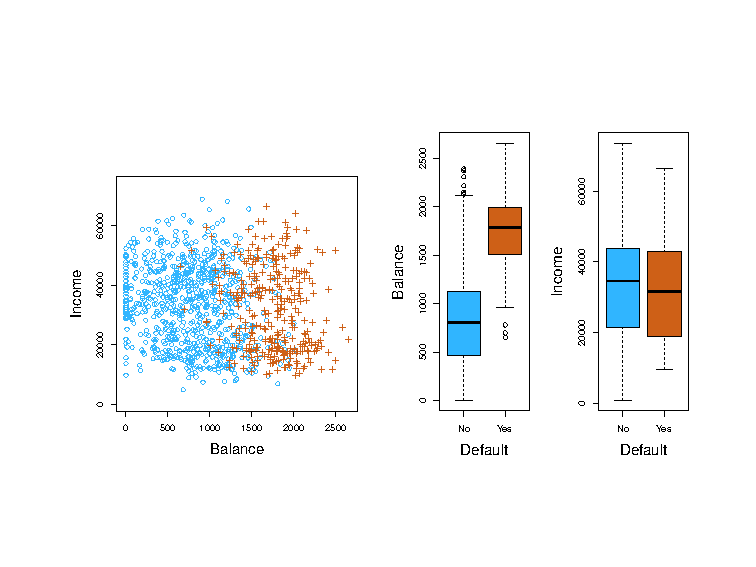
\includegraphics[width=0.65\textwidth]{figures/p02}
\end{frame}

\begin{frame}{Can we use Linear Regression?}
  Suppose for the Default classification task that we code
  \[
    Y = \begin{cases}
      0 & \text{if No} \\
      1 & \text{if Yes.}
    \end{cases}
  \]
  Can we simply perform a linear regression of $Y$ on $X$ and classify as Yes if $\hat{Y} > 0.5$?
  \begin{itemize}
    \item In this case of a binary outcome, linear regression does a good job as a classifier, and is equivalent to linear discriminant analysis which we discuss later.
    \item Since in the population $\text{E}(Y \mid X = x) = \Pr(Y = 1 \mid X = x)$, we might think that regression is perfect for this task.
    \item However, linear regression might produce probabilities less than zero or bigger than one. Logistic regression is more appropriate.
  \end{itemize}
\end{frame}

\begin{frame}{Linear versus Logistic Regression}
  \centering
  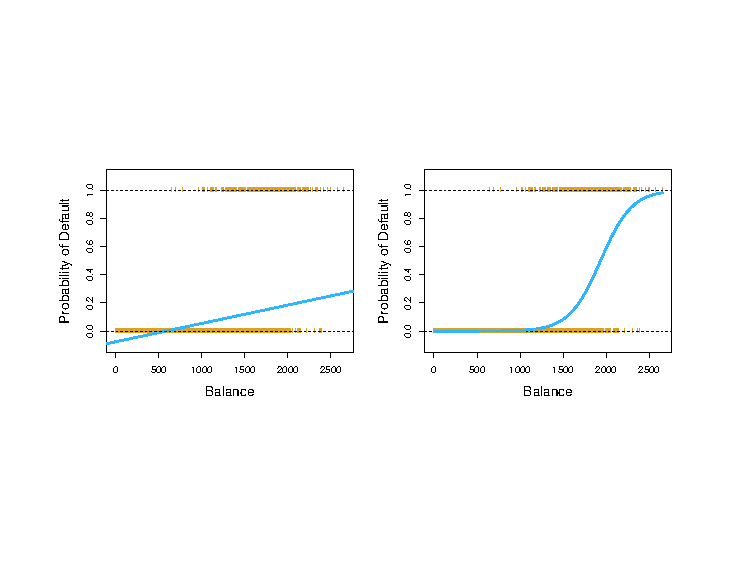
\includegraphics[width=0.75\textwidth]{figures/p04} \\
  \small
  \textbf{Linear vs. Logistic Regression Fits for Binary Data:}
  \begin{itemize}
    \item \textbf{Left (Linear Regression):} A straight regression line fitted to binary 0/1 data results in predicted probabilities that dip below $0.0$ for low balances and exceed $1.0$ for high balances.
    \item \textbf{Right (Logistic Regression):} The S-shaped logistic curve naturally asymptotes at $0.0$ and $1.0$, guaranteeing sensible probability estimates $\Pr(Y = 1 \mid X) \in [0, 1]$ everywhere.
  \end{itemize}
\end{frame}

\begin{frame}{Linear Regression continued}
  Now suppose we have a response variable with three possible values. A patient presents at the emergency room, and we must classify them according to their symptoms:
  \[
    Y = \begin{cases}
      1 & \text{if stroke;} \\
      2 & \text{if drug overdose;} \\
      3 & \text{if epileptic seizure.}
    \end{cases}
  \]
  \begin{itemize}
    \item This coding suggests an ordering, and in fact implies that the difference between stroke and drug overdose is the same as between drug overdose and epileptic seizure.
    \item Linear regression is not appropriate here.
    \item Multiclass Logistic Regression or Discriminant Analysis are more appropriate.
  \end{itemize}
\end{frame}

\section{Logistic Regression}

\begin{frame}{Logistic Regression}
  Let's write $p(X) = \Pr(Y = 1 \mid X)$ for short and consider using \texttt{balance} to predict \texttt{default}. Logistic regression uses the form:
  \[
    p(X) = \frac{e^{\beta_0 + \beta_1 X}}{1 + e^{\beta_0 + \beta_1 X}}.
  \]
  ($e \approx 2.71828$ is Euler's number.)
  \begin{itemize}
    \item It is easy to see that no matter what values $\beta_0, \beta_1$ or $X$ take, $p(X)$ will have values between 0 and 1.
    \item A bit of rearrangement gives:
    \[
      \log\left(\frac{p(X)}{1 - p(X)}\right) = \beta_0 + \beta_1 X.
    \]
    \item This monotone transformation is called the \textbf{log odds} or \textbf{logit} transformation of $p(X)$ (by $\log$ we mean natural log: $\ln$).
  \end{itemize}
\end{frame}

\begin{frame}{Maximum Likelihood}
  We use \textbf{maximum likelihood} to estimate the parameters:
  \[
    \ell(\beta_0, \beta_1) = \prod_{i: y_i = 1} p(x_i) \prod_{i: y_i = 0} (1 - p(x_i)).
  \]
  \begin{itemize}
    \item $p(x_i) = \Pr(Y=1 \mid X=x_i)$: The predicted probability that individual $i$ defaults.
    \item First Product ($\prod_{i: y_i = 1} p(x_i)$): Multiplies the predicted probabilities for all individuals who actually defaulted ($y_i = 1$).
    \item Second Product ($\prod_{i: y_i = 0} (1 - p(x_i))$): Multiplies the predicted probabilities of not defaulting ($1 - p(x_i)$) for all individuals who did not default ($y_i = 0$).
    \item \textbf{Meaning}: The likelihood function represents the joint probability of observing the specific set of zeros and ones present in the dataset.
  \end{itemize}
\end{frame}

\begin{frame}{Maximum Likelihood --continued}
  We use \textbf{maximum likelihood} to estimate the parameters:
  \[
    \ell(\beta_0, \beta_1) = \prod_{i: y_i = 1} p(x_i) \prod_{i: y_i = 0} (1 - p(x_i)).
  \]
  \begin{itemize}
    \item This likelihood gives the probability of the observed zeros and ones in the data. We pick $\beta_0$ and $\beta_1$ to maximize the likelihood of the observed data.
    \item In R we use the \texttt{glm} function with \texttt{family = binomial}.
  \end{itemize}
  \vspace{0.2cm}
  \begin{table}
    \centering
    \small
    \begin{tabular}{l c c c c}
      \toprule
      & \textbf{Coefficient} & \textbf{Std. Error} & \textbf{$Z$-statistic} & \textbf{$P$-value} \\
      \midrule
      \textbf{Intercept} & -10.6513 & 0.3612 & -29.5 & $< 0.0001$ \\
      \textbf{balance}   &   0.0055 & 0.0002 &  24.9 & $< 0.0001$ \\
      \bottomrule
    \end{tabular}
  \end{table}
\end{frame}

\begin{frame}{Hypothesis Testing: $z$-statistic vs. $t$-statistic}
\begin{columns}[T]
    \begin{column}{0.48\textwidth}
        \begin{block}{Linear Regression (Chapter 3)}
            \begin{itemize}
                \item \textbf{Fitting Method:} Ordinary Least Squares (OLS).
                \item \textbf{Error Variance ($\sigma^2$):} Unknown and must be estimated from data via Residual Standard Error (RSE).
                \item \textbf{Exact Distribution:} Under normality of errors, dividing by the estimated SE yields an exact \textbf{Student's $t$-distribution}:
                $$t = \frac{\hat{\beta}_j - 0}{\text{SE}(\hat{\beta}_j)} \sim t_{n-p-1}$$
            \end{itemize}
        \end{block}
    \end{column}

    \begin{column}{0.48\textwidth}
        \begin{block}{Logistic Regression (Chapter 4)}
            \begin{itemize}
                \item \textbf{Fitting Method:} Maximum Likelihood Estimation (MLE).
                \item \textbf{Variance Determined:} For binary outcomes, $\text{Var}(Y|X) = p(X)(1 - p(X))$; there is no separate $\sigma^2$ parameter.
                \item \textbf{Asymptotic Normality:} By MLE theory (large samples), the Wald statistic follows a \textbf{standard normal distribution}:
                $$z = \frac{\hat{\beta}_j - 0}{\text{SE}(\hat{\beta}_j)} \sim \mathcal{N}(0, 1)$$
            \end{itemize}
        \end{block}
    \end{column}
\end{columns}

\vspace{0.25cm}
\begin{alertblock}{Key Takeaway}
$t$-tests account for the additional uncertainty of estimating the unknown error variance $\sigma^2$ in finite samples. MLE in logistic regression relies directly on large-sample asymptotic normality ($z$-test).
\end{alertblock}
\end{frame}

\begin{frame}{Making Predictions}
  \begin{itemize}
    \item What is our estimated probability of default for someone with a balance of \$1000?
    \[
      \hat{p}(X) = \frac{e^{\hat{\beta}_0 + \hat{\beta}_1 X}}{1 + e^{\hat{\beta}_0 + \hat{\beta}_1 X}} = \frac{e^{-10.6513 + 0.0055 \times 1000}}{1 + e^{-10.6513 + 0.0055 \times 1000}} = 0.006
    \] \pause
    \item With a balance of \$2000?
    \[
      \hat{p}(X) = \frac{e^{\hat{\beta}_0 + \hat{\beta}_1 X}}{1 + e^{\hat{\beta}_0 + \hat{\beta}_1 X}} = \frac{e^{-10.6513 + 0.0055 \times 2000}}{1 + e^{-10.6513 + 0.0055 \times 2000}} = 0.586
    \]
  \end{itemize}
\end{frame}

\begin{frame}{Using \texttt{student} as the Predictor}
  Let's fit a logistic regression model with \texttt{student} as the single predictor:
  \begin{table}
    \centering
    \small
    \begin{tabular}{l c c c c}
      \toprule
      & \textbf{Coefficient} & \textbf{Std. Error} & \textbf{$Z$-statistic} & \textbf{$P$-value} \\
      \midrule
      \textbf{Intercept}    & -3.5041 & 0.0707 & -49.55 & $< 0.0001$ \\
      \textbf{student[Yes]} &  0.4049 & 0.1150 &   3.52 &   0.0004   \\
      \bottomrule
    \end{tabular}
  \end{table}
  \vspace{0.2cm}
  Predicted probabilities:
  \begin{align*}
    \widehat{\Pr}(\text{default} = \text{Yes} \mid \text{student} = \text{Yes}) &= \frac{e^{-3.5041 + 0.4049 \times 1}}{1 + e^{-3.5041 + 0.4049 \times 1}} = 0.0431, \\
    \widehat{\Pr}(\text{default} = \text{Yes} \mid \text{student} = \text{No})  &= \frac{e^{-3.5041 + 0.4049 \times 0}}{1 + e^{-3.5041 + 0.4049 \times 0}} = 0.0292.
  \end{align*}
\end{frame}

\begin{frame}{Logistic Regression with Several Variables}
  \[
    \log\left(\frac{p(X)}{1 - p(X)}\right) = \beta_0 + \beta_1 X_1 + \dots + \beta_p X_p \implies p(X) = \frac{e^{\beta_0 + \beta_1 X_1 + \dots + \beta_p X_p}}{1 + e^{\beta_0 + \beta_1 X_1 + \dots + \beta_p X_p}}
  \]
  \begin{table}
    \centering
    \small
    \begin{tabular}{l c c c c}
      \toprule
      & \textbf{Coefficient} & \textbf{Std. Error} & \textbf{$Z$-statistic} & \textbf{$P$-value} \\
      \midrule
      \textbf{Intercept}    & -10.8690 & 0.4923 & -22.08 & $< 0.0001$ \\
      \textbf{balance}      &   0.0057 & 0.0002 &  24.74 & $< 0.0001$ \\
      \textbf{income}       &   0.0030 & 0.0082 &   0.37 &   0.7115   \\
      \textbf{student[Yes]} &  -0.6468 & 0.2362 &  -2.74 &   0.0062   \\
      \bottomrule
    \end{tabular}
  \end{table}
  \vspace{0.2cm}
  \textit{Why is the coefficient for \texttt{student} negative now, while it was positive in the simple model?}
\end{frame}

\begin{frame}{Confounding in the Credit Card Data}
  \centering
  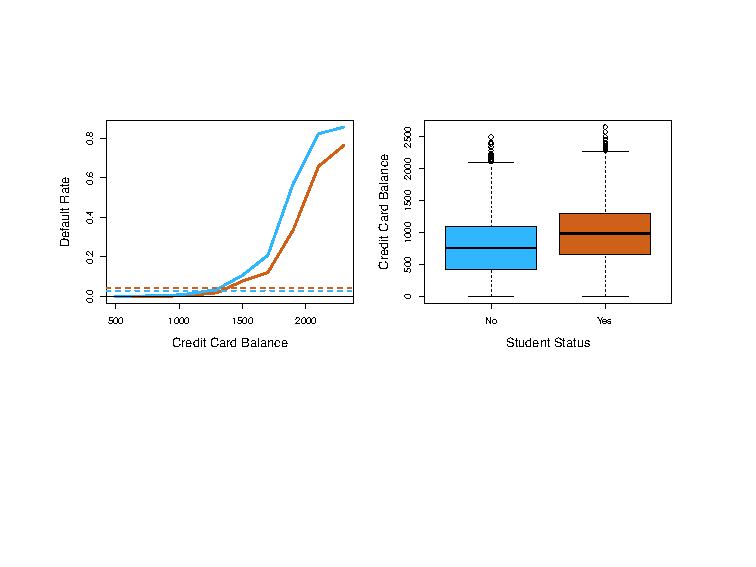
\includegraphics[width=0.75\textwidth]{figures/p12} \\
  {\tiny \textbf{Confounding Phenomenon (Simpson's Paradox):} \textbf{Left (Default Rate vs. Balance):} For any given credit card balance level, students (orange line) have a lower default rate than non-students (blue line). \textbf{Right (Student vs. Balance Boxplot):} However, students tend to hold substantially higher credit card balances on average compared to non-students.}
  \begin{itemize}
    \footnotesize
    \item Students have higher overall (marginal) default rate because they carry more debt.
    \item But controlling for balance, being a student is associated with lower default risk.
    \item Multiple logistic regression teases this out!
  \end{itemize}
\end{frame}

\begin{frame}{The Apparent Contradiction: Marginal vs. Conditional}
\begin{itemize}
    \item \textbf{Scenario:} We want to predict whether an individual will \texttt{Default} on credit card debt using \texttt{Student} status ($1 = \text{Yes}, 0 = \text{No}$) and \texttt{Balance}.
\end{itemize}

\vspace{-0.2cm}
\footnotesize
\begin{columns}[T]
    \begin{column}{0.48\textwidth}
        \begin{block}{Simple Logistic Regression (Marginal)}
            $$\Pr(\text{Def} = \text{Yes}) = \frac{e^{\beta_0 + \beta_1 \cdot \text{Stu}}}{1 + e^{\beta_0 + \beta_1 \cdot \text{Stu}}}$$
            \begin{itemize}
                \item $\hat{\beta}_1 = +0.405$ ($p < 0.001$, positive)
                \item \textbf{Interpretation:} Students are \textbf{more likely} to default overall than non-students ($4.3\%$ vs $2.9\%$).
            \end{itemize}
        \end{block}
    \end{column}

    \begin{column}{0.48\textwidth}
        \begin{block}{Multiple Logistic Regression (Conditional)}
            $$\Pr(\text{Def} = \text{Yes}) = \frac{e^{\beta_0 + \beta_1 \text{Stu} + \beta_2 \text{Bal} + \beta_3 \text{Inc}}}{1 + e^{\cdots}}$$
            \begin{itemize}
                \item $\hat{\beta}_1 = -0.647$ ($p = 0.006$, negative!)
                \item \textbf{Interpretation:} For a \textbf{fixed balance}, students are \textbf{less likely} to default.
            \end{itemize}
        \end{block}
    \end{column}
\end{columns}

\vspace{0.2cm}
\begin{alertblock}{The Core Question}
    Why does the sign of $\hat{\beta}_{\text{Student}}$ flip from \textbf{positive} to \textbf{negative}?
\end{alertblock}
\end{frame}

\begin{frame}{The Mechanism: Confounding via Debt Balance}
The reversal of sign is driven by the relationship between the predictor variables:

\begin{enumerate}
    \item \textbf{Balance is the Dominant Risk Factor:}
    \begin{itemize}
        \item Higher credit card balance dramatically increases the probability of default ($\hat{\beta}_{\text{Balance}} > 0$).
    \end{itemize}
    \item \textbf{Correlation Between Student Status and Balance:}
    \begin{itemize}
        \item Students systematically carry \textbf{higher average balances} than non-students.
    \end{itemize}
    \item \textbf{Holding Balance Fixed (Conditional Comparison):}
    \begin{itemize}
        \item When comparing a student and a non-student with the \emph{same} balance, the student's probability of default is actually lower.
    \end{itemize}
\end{enumerate}

\vspace{0.1cm}
\begin{tcolorbox}[colback=blue!5!white,colframe=blue!75!black,title=Confounding / Simpson's Paradox Summary]
In simple regression, \texttt{Student} absorbs the omitted effect of \texttt{Balance}. Once \texttt{Balance} is controlled for in multiple regression, the true conditional effect of \texttt{Student} is revealed.
\end{tcolorbox}
\end{frame}

\begin{frame}{Practical Takeaways for Credit Scoring \& Inference}
\begin{columns}[T]
    \begin{column}{0.48\textwidth}
        \begin{block}{Decision-Making Scenarios}
            \begin{itemize}
                \item \textbf{Balance is Unknown:}
                Students are riskier applicants on average $\Rightarrow$ issue lower credit or higher interest.
                \item \textbf{Balance is Known:}
                A student with balance $\$b$ is \textbf{less risky} than a non-student with the same balance $\$b$.
            \end{itemize}
        \end{block}
    \end{column}

    \begin{column}{0.48\textwidth}
        \begin{block}{Key Statistical Lessons}
            \begin{itemize}
                \item \textbf{Omitted Variable Bias:} Marginal associations can be severely misleading when key confounders are omitted.
                \item \textbf{Multivariate Modeling:} Coefficients represent effects \emph{holding other variables constant}.
                \item \textbf{Correlation $\neq$ Causation:} Always consider the joint distribution of predictors.
            \end{itemize}
        \end{block}
    \end{column}
\end{columns}
\end{frame}

\begin{frame}{Example: South African Heart Disease}
  \begin{itemize}
    \item 160 cases of MI (myocardial infarction) and 302 controls (all male in age range 15--64), from Western Cape, South Africa in the early 1980s.
    \item Overall prevalence is very high in this region: 5.1\%.
    \item Measurements on seven predictors (risk factors): \texttt{sbp} (systolic blood pressure), \texttt{tobacco}, \texttt{ldl} (low density lipoprotein cholesterol), \texttt{famhist} (family history of heart disease), \texttt{obesity}, \texttt{alcohol}, and \texttt{age}.
    \item Goal is to identify relative strengths and directions of risk factors.
    \item Part of an intervention study aimed at educating the public on healthier diets.
  \end{itemize}
\end{frame}

\begin{frame}{South African Heart Disease: Scatterplot Matrix}
  \begin{columns}[c]
    \begin{column}{0.48\textwidth}
      \centering
      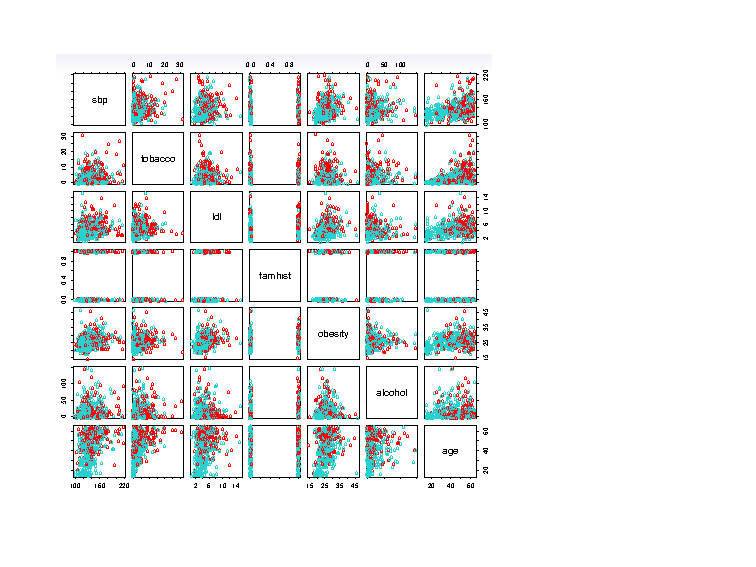
\includegraphics[width=\linewidth]{figures/p14}\\
    \end{column}
    \begin{column}{0.48\textwidth}
      Scatterplot matrix of the South African Heart Disease data. The response is color coded ---the cases (MI) are red, and the controls are turquoise. \texttt{famhist} is a binary variable, with 1 indicating family history of MI.
    \end{column}
  \end{columns}
\end{frame}

\begin{frame}[fragile]{SA Heart Disease: Logistic Regression Model Output}
%   \begin{minted}[fontsize=\footnotesize]{r}
% > heartfit <- glm(chd ~ ., data = heart, family = binomial)
% > summary(heartfit)
% Coefficients:
%                 Estimate Std. Error z value Pr(>|z|)
% (Intercept)    -4.1295997  0.9641558  -4.283 1.84e-05 ***
% sbp             0.0057607  0.0056326   1.023  0.30643
% tobacco         0.0795256  0.0262150   3.034  0.00242 **
% ldl             0.1847793  0.0574115   3.219  0.00129 **
% famhistPresent  0.9391855  0.2248691   4.177 2.96e-05 ***
% obesity        -0.0345434  0.0291053  -1.187  0.23529
% alcohol         0.0006065  0.0044550   0.136  0.89171
% age             0.0425412  0.0101749   4.181 2.90e-05 ***
% ---
% Null deviance: 596.11 on 461 degrees of freedom
% Residual deviance: 483.17 on 454 degrees of freedom; AIC: 499.17
%   \end{minted}

 \centering
 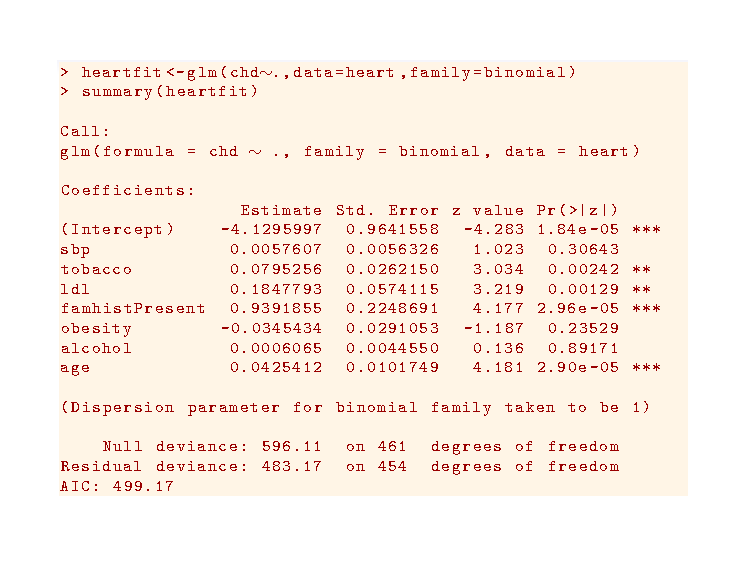
\includegraphics[width=0.75\textwidth]{figures/p15}
\end{frame}

\begin{frame}{Case-Control Sampling and Logistic Regression}
  \begin{itemize}
    \item In the SA data, there are 160 cases and 302 controls ($\tilde{\pi} = 0.35$ cases). Yet the true population prevalence is $\pi = 0.05$.
    \item With case-control samples, we can estimate slope parameters $\beta_j$ accurately (if our model is correct); only the constant term $\beta_0$ is biased.
    \item We can correct the estimated intercept by:
    \[
      \hat{\beta}_0^* = \hat{\beta}_0 + \log\left(\frac{\pi}{1 - \pi}\right) - \log\left(\frac{\tilde{\pi}}{1 - \tilde{\pi}}\right)
    \]
    \item Often cases are rare and we take all of them; up to 5 times that number of controls is sufficient.
  \end{itemize}
\end{frame}

\begin{frame}{Diminishing Returns in Unbalanced Binary Data}
  \begin{columns}[c]
    \begin{column}{0.48\textwidth}
      \centering
      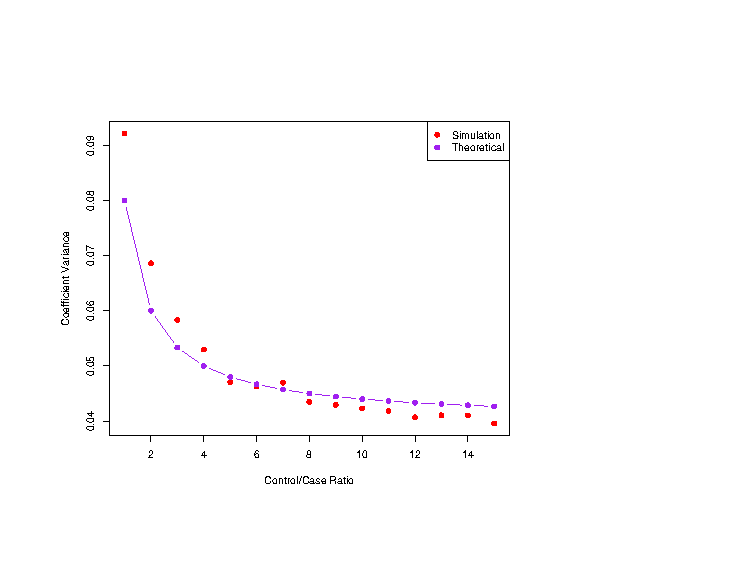
\includegraphics[width=\linewidth]{figures/p17}\\
    \end{column}
    \begin{column}{0.48\textwidth}
    \textbf{Control/Case Ratio vs. Coefficient Variance:} As the control-to-case sampling ratio increases from 1 to 14, the variance of the parameter estimates decreases rapidly up to a ratio of about $5:1$, after which the variance reduction flattens out.
    \end{column}
  \end{columns}
\end{frame}

\begin{frame}{Diminishing Returns in Unbalanced Binary Data --continued}{Motivation \& The Case-Control Design}
    \begin{itemize}
        \item \textbf{The Rare Outcome Challenge:}
        \begin{itemize}
            \item In medical studies (e.g., myocardial infarction), the outcome is rare in the general population ($\pi = \Pr(Y=1) \approx 5\%$).
            \item A simple random sample requires massive sample sizes to observe enough positive cases.
        \end{itemize}
        \vspace{0.5em}
        \item \textbf{Case-Control Strategy:}
        \begin{itemize}
            \item Collect \textbf{all} available cases ($Y=1$) and sample a manageable group of controls ($Y=0$).
        \end{itemize}
        \vspace{0.5em}
        \item \textbf{Proportion Discrepancy (e.g., SA Heart Disease Study):}
        \begin{itemize}
            \item \textbf{Population Prevalence ($\pi$):} $\approx 0.05$ (5.1\% true risk)
            \item \textbf{Sample Proportion ($\tilde{\pi}$):} $\frac{160}{160 + 302} \approx 0.35$ (35\% in sample)
        \end{itemize}
        \vspace{0.5em}
        \item \textbf{Key Question:} Does artificially inflating cases distort parameter estimation?
    \end{itemize}
\end{frame}

\begin{frame}{Diminishing Returns in Unbalanced Binary Data --continued}{Invariance of Slope Estimates}
    \begin{itemize}
        \item \textbf{Log-Odds Representation:}
        \[
            \log\left(\frac{\Pr(Y=1 \mid X)}{1 - \Pr(Y=1 \mid X)}\right) = \beta_0 + \beta_1 X_1 + \dots + \beta_p X_p
        \]
        \item \textbf{Mathematical Invariance Property:}
        \begin{itemize}
            \item Under case-control sampling, the relationship between features $X$ and the outcome $Y$ is preserved.
            \item The estimated slope coefficients $\hat{\beta}_1, \hat{\beta}_2, \dots, \hat{\beta}_p$ are \textbf{unbiased} and match population log-odds ratios.
        \end{itemize}
        \vspace{0.5em}
        \item \textbf{The Catch:}
        \begin{itemize}
            \item Only the intercept term $\beta_0$ is biased upward because it absorbs the inflated baseline rate of cases.
        \end{itemize}
    \end{itemize}
\end{frame}

\begin{frame}{Diminishing Returns in Unbalanced Binary Data --continued}{Intercept Correction for True Probabilities}
    \begin{itemize}
        \item \textbf{Why Correct the Intercept?}
        \begin{itemize}
            \item Unadjusted predictions overestimate the true risk of disease in the population.
        \end{itemize}
        \vspace{0.3em}
        \item \textbf{Correction Formula (when true prevalence $\pi$ is known):}
        \[
            \hat{\beta}_{0}^{*} = \hat{\beta}_{0} + \log\left(\frac{\pi}{1-\pi}\right) - \log\left(\frac{\tilde{\pi}}{1-\tilde{\pi}}\right)
        \]
        \begin{itemize}
            \item $\log\left(\frac{\pi}{1-\pi}\right)$: Log-odds of the disease in the \textbf{population}.
            \item $\log\left(\frac{\tilde{\pi}}{1-\tilde{\pi}}\right)$: Log-odds of the disease in the \textbf{case-control sample}.
        \end{itemize}
        \vspace{0.3em}
        \item \textbf{Calibrated Population Posterior Probabilities:}
        \[
            \widehat{\Pr}(Y=1 \mid X) = \frac{e^{\hat{\beta}_{0}^{*} + \sum_{j=1}^p \hat{\beta}_j X_j}}{1 + e^{\hat{\beta}_{0}^{*} + \sum_{j=1}^p \hat{\beta}_j X_j}}
        \]
    \end{itemize}
\end{frame}

\begin{frame}{Diminishing Returns in Unbalanced Binary Data --continued}{Practical Takeaways \& The 5:1 Sampling Rule}
    \begin{columns}[T]
        \begin{column}{0.55\textwidth}
            \textbf{Key Takeaways:}
            \begin{itemize}
                \item \textbf{Sample Efficiency:} For rare outcomes, case-control sampling dramatically cuts data collection costs without sacrificing slope accuracy.
                \item \textbf{Diminishing Returns:} Increasing the control-to-case ratio beyond $\approx 5:1$ yields negligible variance reduction.
                \item \textbf{Classification vs. Odds:} Odds ratios are valid immediately; correct $\beta_0$ only when absolute probability is needed.
            \end{itemize}
        \end{column}

        \begin{column}{0.42\textwidth}
            \begin{block}{Control-to-Case Ratio}
                \begin{itemize}
                    \item \textbf{1:1 to 4:1:} Steep decrease in parameter variance $\text{Var}(\hat{\beta}_j)$.
                    \item \textbf{$\ge$ 5:1:} Variance curve flattens out.
                    \item \textbf{Rule of Thumb:} Up to 5 controls per case is sufficient in practice.
                \end{itemize}
            \end{block}
        \end{column}
    \end{columns}
\end{frame}

\begin{frame}{Logistic Regression with More than Two Classes}
  \begin{itemize}
    \item Generalizes naturally to $K > 2$ classes (Multinomial Logistic Regression).
    \item Symmetric (softmax) formulation:
    \[
      \Pr(Y = k \mid X) = \frac{e^{\beta_{0k} + \beta_{1k} X_1 + \dots + \beta_{pk} X_p}}{\sum_{\ell=1}^K e^{\beta_{0\ell} + \beta_{1\ell} X_1 + \dots + \beta_{p\ell} X_p}}
    \]
    \item Here there is a linear function for \textbf{each} class.
    \item Redundancy: only $K - 1$ linear functions are required (one class serves as baseline).
    \item Multiclass logistic regression is also referred to as \textbf{multinomial regression}.
  \end{itemize}
\end{frame}

\section{Linear Discriminant Analysis}

\begin{frame}{Discriminant Analysis}
  \begin{itemize}
    \item \textbf{Generative approach:} Model the distribution of $X$ in each of the classes separately ($f_k(x)$), and then use \textbf{Bayes' theorem} to flip things around to obtain $\Pr(Y \mid X)$.
    \item When we use normal (Gaussian) distributions for each class, this leads to linear or quadratic discriminant analysis according to the covariance matrix:
    \begin{itemize}
      \item Common  $\mathbf{\Sigma} \implies$ \textbf{Linear Discriminant Analysis (LDA)}.
      \item Class-specific  $\mathbf{\Sigma}_k \implies$ \textbf{Quadratic Discriminant Analysis (QDA)}.
    \end{itemize}
    \item However, this approach is quite general, and other distributions can be used as well. We will focus on normal distributions.
  \end{itemize}
\end{frame}


\begin{frame}{Bayes' Theorem for Classification}
  \begin{itemize}
    \item Thomas Bayes was a famous mathematician whose name represents a big subfield of statistical and probabilistic modeling. Here we focus on a simple result, known as Bayes theorem:
      \[
        \Pr(Y = k \mid X = x) = \frac{\Pr(X = x \mid Y = k) \cdot \Pr(Y = k)}{\Pr(X = x)}
      \]
    \item For discriminant analysis, this is written as:
      \[
        p_k(x) = \Pr(Y = k \mid X = x) = \frac{\pi_k f_k(x)}{\sum_{\ell=1}^K \pi_\ell f_\ell(x)}
      \]
      where:
      \begin{itemize}
        \item $f_k(x) = \Pr(X = x \mid Y = k)$ is the \textbf{class-conditional density} for $X$ in class $k$.
        \item $\pi_k = \Pr(Y = k)$ is the marginal or \textbf{prior probability} for class $k$.
      \end{itemize}
  \end{itemize}
\end{frame}

\begin{frame}{Classify to the Highest Density}
  \begin{block}{}
    \textbf{1D Densities and Bayes Decision Boundary:}
    \begin{itemize}
      \item \textbf{Equal Priors ($\pi_1 = 0.5, \pi_2 = 0.5$):} Decision boundary is at the point where the two density curves intersect ($x = (\mu_1 + \mu_2)/2$).
      \item \textbf{Unequal Priors ($\pi_1 = 0.3, \pi_2 = 0.7$):} The decision boundary shifts toward class 1 (left) to favor the higher prior probability of class 2.
    \end{itemize}
  \end{block}
  \centering
  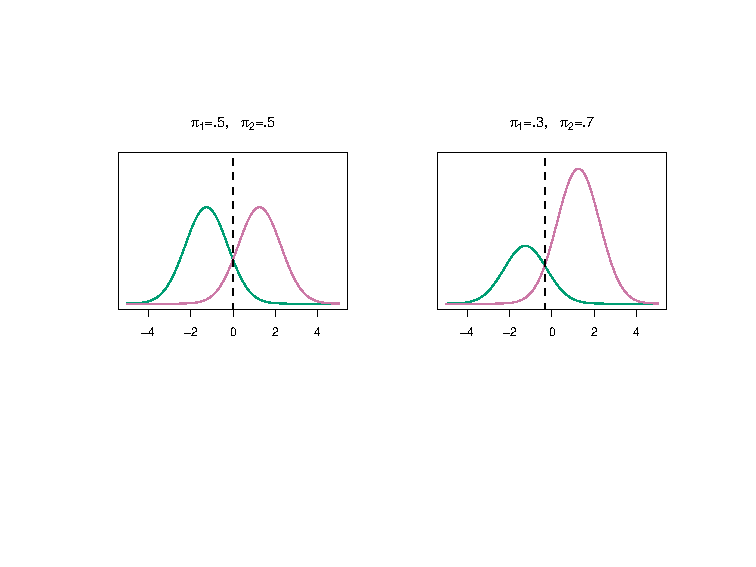
\includegraphics[width=0.6\textwidth]{figures/p21}
\end{frame}

\begin{frame}{Why Discriminant Analysis?}
  \begin{itemize}
    \item \textbf{Separation problem:} When classes are well-separated, logistic regression parameter estimates are surprisingly unstable (coefficients diverge to $\pm \infty$). LDA does not suffer from this.
    \item \textbf{Small sample size:} If $n$ is small and the distribution of predictors is approximately Gaussian in each class, LDA is more stable and efficient than logistic regression.
    \item \textbf{Multiclass ($K > 2$):} LDA provides convenient low-dimensional visualizations and projections of the data.
  \end{itemize}
\end{frame}

\begin{frame}{Linear Discriminant Analysis when $p = 1$}
  The Gaussian (normal) density has the form:
  \[
    f_k(x) = \frac{1}{\sqrt{2\pi}\sigma_k} e^{-\frac{1}{2}\left(\frac{x - \mu_k}{\sigma_k}\right)^2}
  \]
  Here $\mu_k$ is the mean, and $\sigma_k^2$ the variance (in class $k$). We will assume that all the $\sigma_k = \sigma$ are the same ($\sigma_1^2 = \dots = \sigma_k^2 = \sigma^2$).  \\
  \pause

  So,  Bayes' formula gives us a rather complex expression for $p_k(x) = Pr(Y = k|X = x)$:
  \[
    p_k(x) = \frac{\pi_k \frac{1}{\sqrt{2\pi}\sigma} e^{-\frac{1}{2}\left(\frac{x - \mu_k}{\sigma_k}\right)^2}}{\sum_{\ell=1}^K \pi_\ell \frac{1}{\sqrt{2\pi}\sigma} e^{-\frac{1}{2}\left(\frac{x - \mu_k}{\sigma_k}\right)^2}}
  \]
  \pause
  Happily, there are simplifications and cancellations.
\end{frame}

\begin{frame}{Discriminant Functions ($p=1$)}
  Taking logs and removing common constants, maximizing $p_k(x)$ is equivalent to maximizing the \textbf{linear discriminant score}:
  \[
    \delta_k(x) = x \cdot \frac{\mu_k}{\sigma^2} - \frac{\mu_k^2}{2\sigma^2} + \log(\pi_k)
  \]
  \begin{itemize}
    \item Note that $\delta_k(x)$ is a \textbf{linear} function of $x$. \pause
    \item For $K = 2$ classes and equal priors ($\pi_1 = \pi_2 = 0.5$), the \textbf{decision boundary} ($\delta_1(x) = \delta_2(x)$) is:
    \[
      x = \frac{\mu_1 + \mu_2}{2}
    \]
  \end{itemize}
\end{frame}

\begin{frame}{Discriminant Functions ($p=1$) --continued}
  \centering
  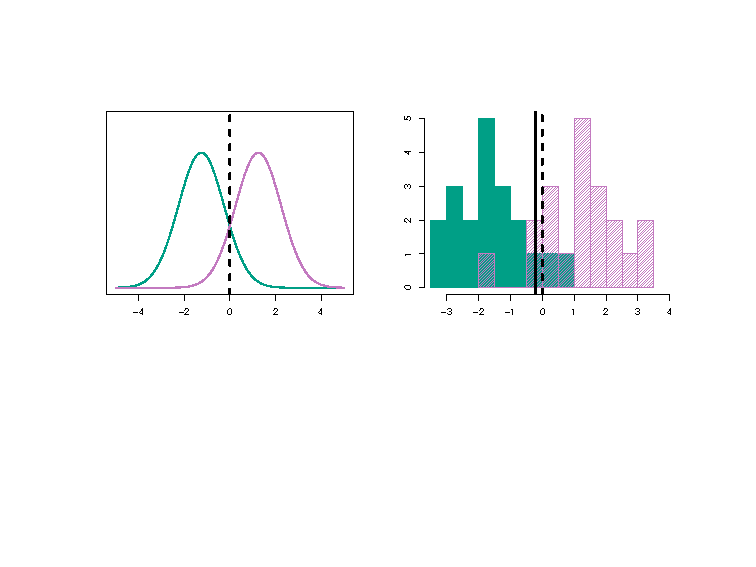
\includegraphics[width=0.9\textwidth]{figures/p25} \\

  \begin{itemize}
      \item Example with $\mu_1 = -1.5$, $\mu_2 = 1.5$, $\pi_1 = \pi_2 = 0.5$, and $\sigma^2 = 1$. \pause
      \item Typically we don’t know these parameters; we just have the training data. In that case we simply estimate the parameters and plug them into the rule.
  \end{itemize}
\end{frame}


\begin{frame}{Estimating the Parameters for LDA}
  In practice, true parameters are unknown and estimated from training data:
  \begin{align*}
    \hat{\pi}_k &= \frac{n_k}{n} \\
    \hat{\mu}_k &= \frac{1}{n_k} \sum_{i: y_i = k} x_i \\
    \hat{\sigma}^2 &= \frac{1}{n - K} \sum_{k=1}^K \sum_{i: y_i = k} (x_i - \hat{\mu}_k)^2 = \sum_{k=1}^K \frac{n_k - 1}{n - K} \hat{\sigma}_k^2
  \end{align*}
  where $\hat{\sigma}_k^2 = \frac{1}{n_k - 1}\sum_{i: y_i = k} (x_i - \hat{\mu}_k)^2$ is the usual formula for the estimated variance in the class $k$.
\end{frame}

\begin{frame}{Linear Discriminant Analysis when $p > 1$}
  \centering
  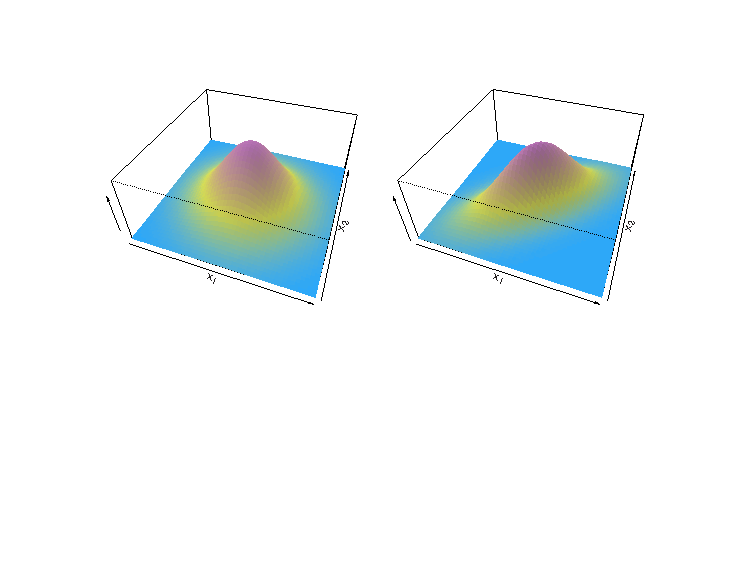
\includegraphics[width=0.9\textwidth]{figures/p27} \\
  Density: $f(x) = \frac{1}{(2\pi)^{\frac{p}{2}}|\mathbf{\Sigma}|^{\frac{1}{2}}}e^{-\frac{1}{2}(x - \mu)^T \mathbf{\Sigma}^{-1} (x - \mu)}$ \\
  \pause
  \begin{itemize}
    \item Discriminant function: $\delta_k(x) = x^T \mathbf{\Sigma}^{-1} \mu_k - \frac{1}{2} \mu_k^T \mathbf{\Sigma}^{-1} \mu_k + \log \pi_k$ \pause
    \item Despite its complex form, $\delta_k(x) = c_{k0} + c_{k1} x_1 + c_{k2} x_2 + \dots + c_{kp} x_p$ is a \textbf{linear function} of $x$.
  \end{itemize}
\end{frame}

\begin{frame}{Illustration: $p = 2$ and $K = 3$ Classes}
  \textbf{2D Gaussian LDA Contours and Decision Boundaries:}
  \begin{itemize}
    \footnotesize
    \item Here we have 3 classes with equal priors ($\pi_1 = \pi_2 = \pi_3 = \frac{1}{3}$).
    \item Elliptical contour lines represent bivariate Gaussian densities with shared covariance $\mathbf{\Sigma}$.
    \item Dashed lines represent optimal \textbf{Bayes decision boundaries} dividing the plane into three polygonal regions.
    \item Were they known, they would yield the fewest misclassification errors, among all possible classifiers.
  \end{itemize}
  \centering
  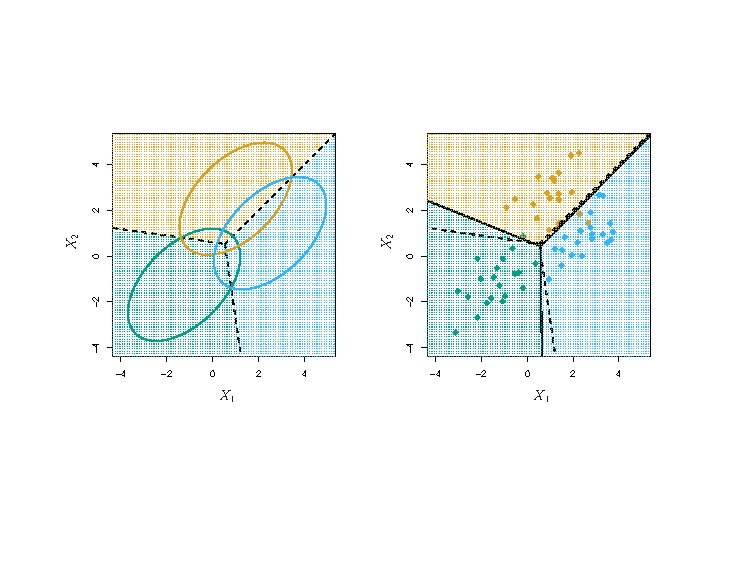
\includegraphics[width=0.7\textwidth]{figures/p28}
\end{frame}

\begin{frame}{Fisher's Iris Data}
  \begin{columns}[c]
    \begin{column}{0.48\textwidth}
      \centering
      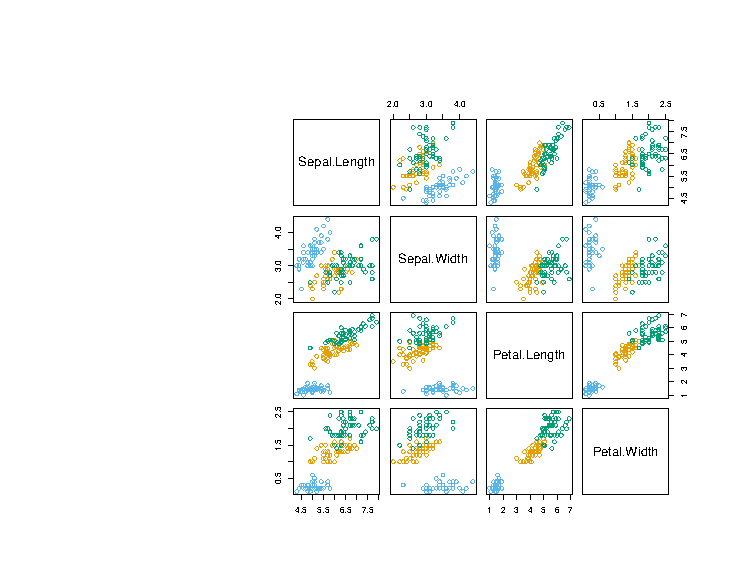
\includegraphics[width=\linewidth]{figures/p29}\\
    \end{column}
    \begin{column}{0.48\textwidth}
      \begin{itemize}
        \item 4 continuous measurements: \texttt{Sepal.Length}, \texttt{Sepal.Width}, \texttt{Petal.Length}, \texttt{Petal.Width}.
        \item 3 species ($K = 3$): \textit{Setosa (blue)}, \textit{Versicolor (orange)}, \textit{Virginica (green)} (50 samples per class, $n = 150$).
        \item LDA correctly classifies all but 3 of the 150 training samples (2\% training error).
      \end{itemize}
    \end{column}
  \end{columns}
\end{frame}

\begin{frame}{Fisher's Discriminant Plot}
  \centering
  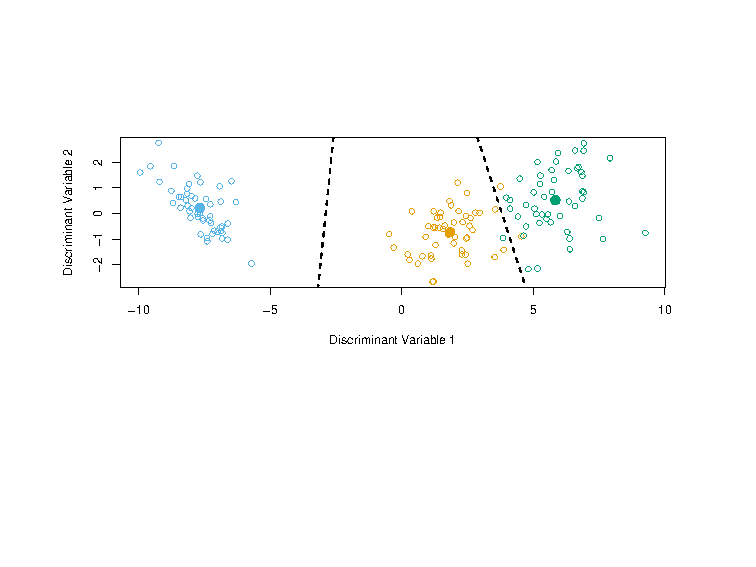
\includegraphics[width=0.8\textwidth]{figures/p30}
  \begin{block}{}
    \textbf{Fisher's Linear Discriminants for Iris Data:}
    \begin{itemize}
      \item When there are K classes, linear discriminant analysis can be viewed exactly in a K - 1 dimensional plot.
      \item Why?
    \end{itemize}
  \end{block}
\end{frame}

\begin{frame}{Fisher's Discriminant Plot}
  \centering
  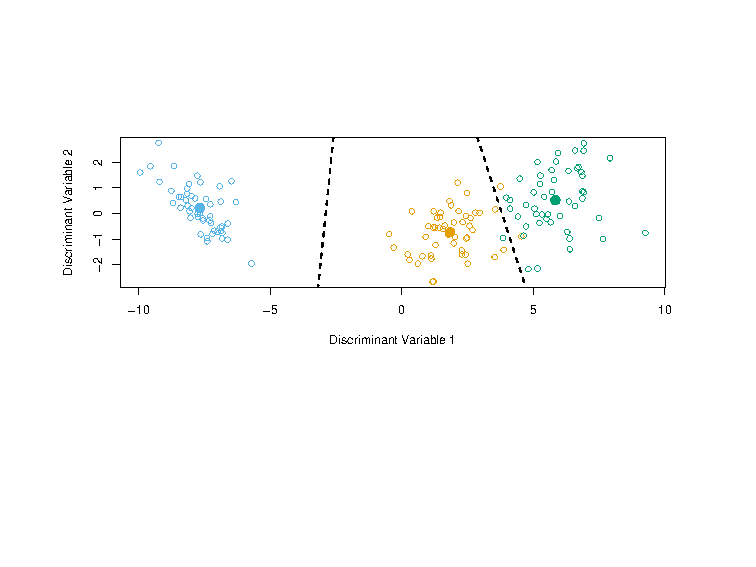
\includegraphics[width=0.8\textwidth]{figures/p30}
  \begin{itemize}
    \item When there are K classes, linear discriminant analysis can be viewed exactly in a $K - 1$ dimensional plot.
    \item \textbf{Why?} Because LDA essentially classifies to the closest centroid in Mahalanobis distance, and $K$ centroids span at most a $(K - 1)$-dimensional hyperplane. \pause
    \item Even when $K > 3$, we can find the ``best'' 2-dimensional plane for visualizing the discriminant rule.
  \end{itemize}
\end{frame}

\begin{frame}{From $\delta_k(x)$ to Class Probabilities}
  Once we have estimates $\hat{\delta}_k(x)$, we convert them into posterior class probabilities:
  \[
    \widehat{\Pr}(Y = k \mid X = x) = \frac{e^{\hat{\delta}_k(x)}}{\sum_{\ell=1}^K e^{\hat{\delta}_\ell(x)}}
  \]
  \begin{itemize}
    \item Classifying to the largest $\hat{\delta}_k(x)$ is identical to classifying to the class with highest posterior probability.
    \item For $K = 2$, we predict class 2 if $\widehat{\Pr}(Y = 2 \mid X = x) \ge 0.5$, else class 1.
  \end{itemize}
\end{frame}

\section{Classification Evaluation \& Other Classifiers}

\begin{frame}{LDA on Credit Data: Confusion Matrix}
  \begin{table}
    \centering
    \begin{tabular}{l c c c c}
      \toprule
      & & \multicolumn{2}{c}{\textbf{True Default Status}} & \\
      \cmidrule(lr){3-4}
      & & \textbf{No} & \textbf{Yes} & \textbf{Total} \\
      \midrule
      \textbf{Predicted} & \textbf{No}  & 9644 & 252 & 9896 \\
      \textbf{Default Status} & \textbf{Yes} & 23   & 81  & 104  \\
      \midrule
      & \textbf{Total} & 9667 & 333 & 10000 \\
      \bottomrule
    \end{tabular}
  \end{table}
  \vspace{0.2cm}
  $\frac{23 + 252}{10000} = \frac{275}{10000}$ errors --an apparent \textit{misclassification rate} of $2.75\%$.
  \pause
  \begin{itemize}
    \item A trivial \textbf{null classifier} (always predicting No) has an error rate of $333/10000 = 3.33\%$.
    \item \textbf{False Positive Rate (True \texttt{No}'s errors):} $\frac{23}{9667} = 0.2\%$ .
    \item \textbf{False Negative Rate (True \texttt{Yes}'s errors):} $\frac{252}{333} = 75.7\%$ (missed 75.7\% of defaults!).
  \end{itemize}
\end{frame}

\begin{frame}{Types of Errors \& Varying the Threshold}
  \begin{block}{False positive rate:} The fraction of negative examples that are classified as positive $\longrightarrow$ 0.2\% in example.
  \end{block}
  \begin{block}{False negative rate:} The fraction of positive examples that are
classified as negative $\longrightarrow$ 75.7\% in example.
  \end{block}
  \pause
  \begin{itemize}
    \item Defaulting threshold was set at $0.5$: predict default if $\widehat{\Pr}(\text{Default} = \text{Yes} \mid X) \ge 0.5$.
    \item In credit card default, a false negative is much more costly than a false positive.
    \item We can vary the threshold to any value in $[0, 1]$:
    \[
      \widehat{\Pr}(\text{Default} = \text{Yes} \mid X) \ge \text{\textit{threshold}}.
    \]
  \end{itemize}
\end{frame}

\begin{frame}{Types of Errors \& Varying the Threshold --continued}
  \centering
  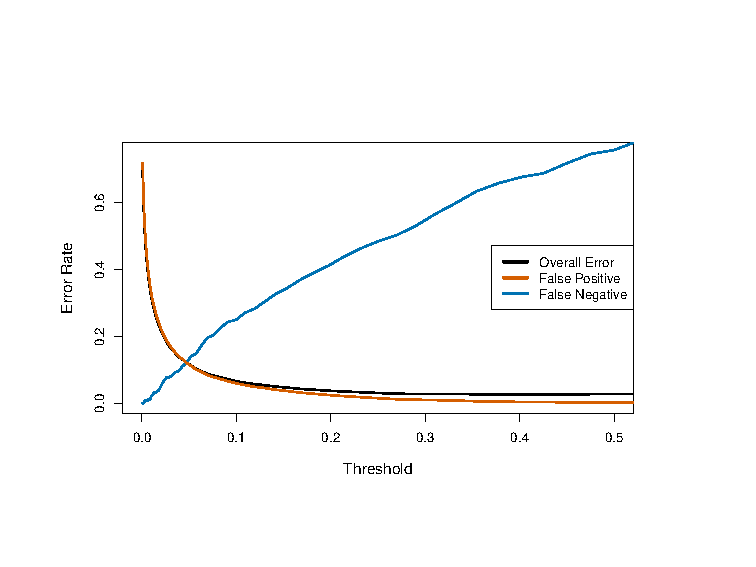
\includegraphics[width=0.8\textwidth]{figures/p34} \\
  \footnotesize
  \textbf{Threshold vs. Error Rates:} Lowering threshold from $0.5$ down to $0.1$ dramatically drops the false negative rate with only a modest increase in false positives and overall error.
\end{frame}

\begin{frame}{ROC Curve}
  \begin{columns}[c]
    \begin{column}{0.48\textwidth}
      \centering
      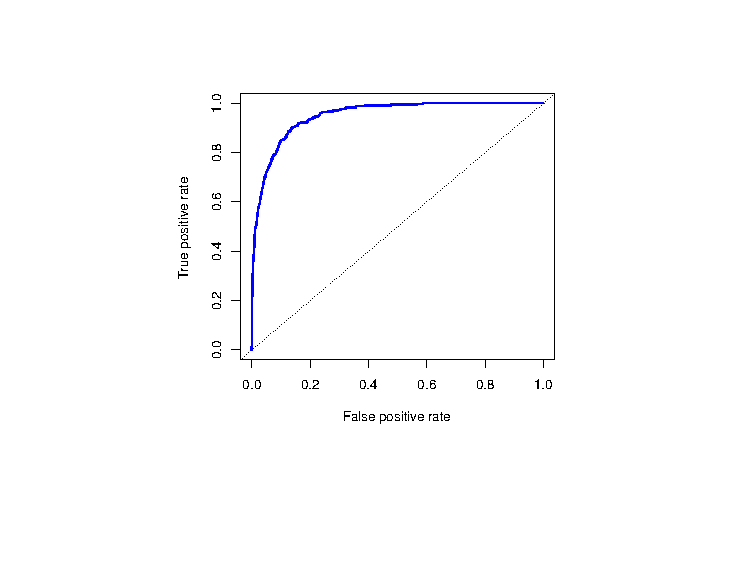
\includegraphics[width=\linewidth]{figures/p35}\\
    \end{column}
    \begin{column}{0.48\textwidth}
      \footnotesize
      \textbf{Receiver Operating Characteristic (ROC) Curve:}
      \begin{itemize}
        \item Displays \textbf{True Positive Rate} (Sensitivity) vs. \textbf{False Positive Rate} ($1 - \text{Specificity}$) across all possible classification thresholds.
        \item An ideal ROC curve hugs the top-left corner.
      \end{itemize}
      \begin{itemize}
        \item The performance is summarized by the \textbf{AUC} (Area Under the ROC Curve).
        \item AUC ranges from $0.5$ (random guessing) to $1.0$ (perfect classification). Higher AUC is better.
      \end{itemize}
    \end{column}
  \end{columns}
\end{frame}

\begin{frame}{Other Forms of Discriminant Analysis}
  Recall Bayes' formula:
  \[
    \Pr(Y = k \mid X = x) = \frac{\pi_k f_k(x)}{\sum_{\ell=1}^K \pi_\ell f_\ell(x)}
  \]
  When $f_k(x)$ are Gaussian densities, with the same covariance matrix $\mathbf{\Sigma}$ in each class, this leads to linear discriminant analysis.  By altering the forms for $f_k(x)$, we get different classifiers.
  \begin{itemize}
    \item \textbf{LDA:} $f_k(x)$ is Gaussian with shared covariance matrix $\mathbf{\Sigma}$.
    \item \textbf{QDA (Quadratic DA):} $f_k(x)$ is Gaussian with \textbf{class-specific} covariance matrices $\mathbf{\Sigma}_k$.
    \item \textbf{Naive Bayes:} $f_k(x) = \prod_{j=1}^p f_{kj}(x_j)$ assumes conditional independence across features within each class (for Gaussian this
means the $\mathbf{\Sigma}_k$ are diagonal).
    \item \textbf{Non-parametric DA:} Uses kernel density estimation or histograms for $f_k(x)$.
  \end{itemize}
\end{frame}

\begin{frame}{Quadratic Discriminant Analysis (QDA)}
  When $\mathbf{\Sigma}_k$ are distinct for each class $k$, the quadratic terms no longer cancel:
  \[
    \delta_k(x) = -\frac{1}{2}(x - \mu_k)^T \mathbf{\Sigma}_k^{-1}(x - \mu_k) - \frac{1}{2}\log|\mathbf{\Sigma}_k| + \log \pi_k
  \]

  \centering
  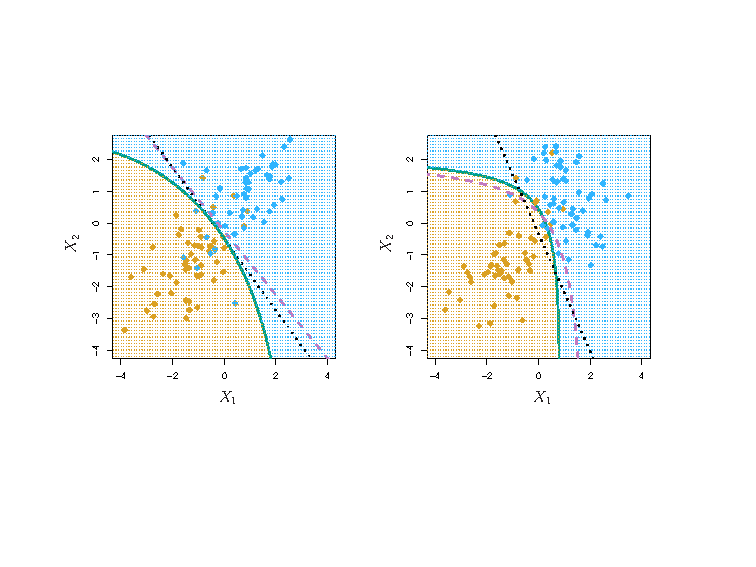
\includegraphics[width=0.7\textwidth]{figures/p37} \\
  \textbf{\footnotesize QDA vs. LDA Decision Boundaries:}
\end{frame}

\begin{frame}{Quadratic Discriminant Analysis (QDA) --continued}
  \centering
  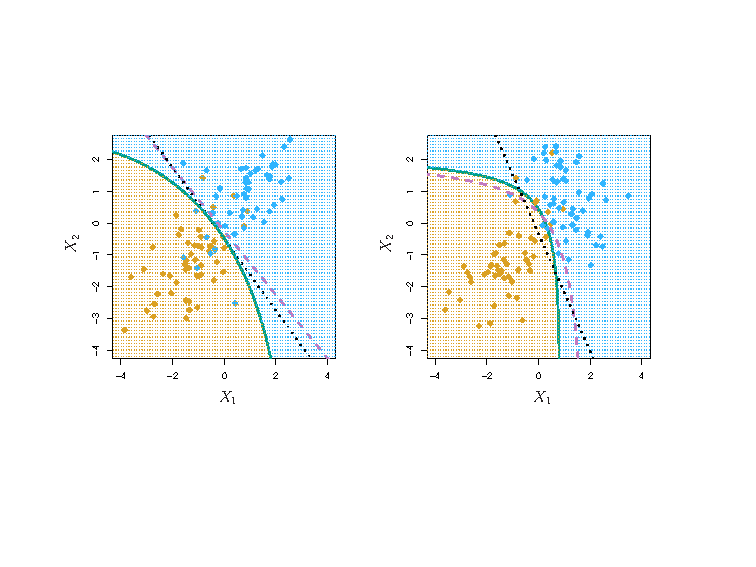
\includegraphics[width=0.7\textwidth]{figures/p37} \\
  \textbf{\footnotesize QDA vs. LDA Decision Boundaries:}
  \begin{itemize}
    \footnotesize
    \item When classes have different correlation structures/variances, the Bayes boundary is curved (quadratic).
    \item QDA fits curved quadratic boundaries, capturing complex interactions at the cost of estimating $K \times p(p+1)/2$ covariance parameters.
  \end{itemize}
\end{frame}

\begin{frame}{Naive Bayes}
  \begin{itemize}
    \item Assumes features are conditionally independent in each class: $f_k(x) = \prod_{j=1}^p f_{kj}(x_j)$.
    \item Useful when $p$ is large (where covariance estimation in LDA/QDA breaks down).
    \item \textbf{Gaussian Naive Bayes:} $\mathbf{\Sigma}_k$ is diagonal ($\sigma_{kj}^2$):
    \[
      \delta_k(x) \propto \log\left[\pi_k \prod_{j=1}^p f_{kj}(x_j)\right] = -\frac{1}{2}\sum_{j=1}^p \left[\frac{(x_j - \mu_{kj})^2}{\sigma_{kj}^2} + \log \sigma_{kj}^2\right] + \log \pi_k
    \]
    \item \textbf{Mixed features:} Easily handles qualitative features using discrete probability tables/histograms.
    \item Despite strong independence assumptions, Naive Bayes often performs surprisingly well.
  \end{itemize}
\end{frame}

\begin{frame}{Logistic Regression versus LDA}
  For a two-class problem, the log-odds for LDA is:
  \[
    \log\left(\frac{p_1(x)}{1 - p_1(x)}\right) = \log\left(\frac{p_1(x)}{p_2(x)}\right) = c_0 + c_1 x_1 + \dots + c_p x_p
  \]
  Both models produce linear decision boundaries! The key difference lies in how the parameters are estimated: \pause
  \begin{itemize}
    \item \textbf{Logistic Regression\footnote{Logistic regression can fit non-linear boundaries by explicitly adding polynomial or interaction terms.} (Discriminative learning):} Maximizes conditional likelihood $\Pr(Y \mid X)$. Makes fewer distributional assumptions.
    \item \textbf{LDA (Generative learning):} Maximizes full joint likelihood $\Pr(X, Y)$ assuming Gaussianity. More efficient when normality holds.
    \item Despite these differences, in practice the results are often very similar.
  \end{itemize}
\end{frame}

\begin{frame}{Summary of Classification Methods}
  \begin{itemize}
    \item \textbf{Logistic Regression:} Very popular and robust for binary ($K = 2$) and multiclass problems.
    \item \textbf{LDA:} Well-suited when $n$ is small, classes are well-separated, or normality holds; provides dimension reduction.
    \item \textbf{QDA:} Useful when sample size is large and covariance matrices differ noticeably between classes.
    \item \textbf{Naive Bayes:} Ideal when $p$ is very large or features are mixed categorical/continuous.
    \item \textbf{KNN:} Non-parametric, flexible when decision boundary is highly irregular, but suffers in high dimensions (Section 4.5).
  \end{itemize}
\end{frame}

\end{document}
